\section{Numerical experiments}

To evaluate the simple model of \sref{model}, we conduct a battery of direct numerical simulations of the imcompressible Navier-Stokes equations with the Boussinesq approximation:
\begin{align}
\frac{\partial u}{\partial t} + u \cdot \nabla u &= \nu \nabla^2 u - \nabla P + A g \phi \\
\frac{\partial \phi}{\partial t} + u \cdot \nabla \phi &= D \nabla^2 \phi 
\end{align}
where $u$ is the velocity,
$\nu$ is the kinematic viscosity,
$P$ is the pressure,
$\phi$ the non-dimensional density,
and $D$ is the diffusivity of $\phi$.

The initial conditions are quicent with a horizontal interface perturbed by product of cosine functions and smeared by an error function:
\begin{equation}
\phi(x,y,z,t=0) = \text{erf}\left(\frac{z + a_0 \cos(2 \pi (x/\lambda)) \cos(2 \pi (y/\lambda))}{\delta})\right)
\end{equation}
where $a_0$ is the initial amplitude and $\delta$ is the initial interface thickness.
Both $a_0$ and $\delta$ are taken to be small enough to minimize their effects on the solution, $0.01$ and $1/???$, respectively.
The governing equations and initial condition have four dimensional parameters: $\nu$, $D$, $Ag$, $\lambda$.
These are combined into 2 non-dimensional numbers, the Grashof number and the Schmidt number:
\begin{equation}
\text{Gr} = \frac{A g \lambda^3}{\nu^2} \quad \text{Sc} = \frac{\nu}{D}
\end{equation}
The Grashof number serves the role of a Reynolds number for instability problems without a consistent characteristic velocity.
For this reason, the root of the Grashof number is sometimes called the \textit{perturbation Reynolds number}~\cite{Wei2011}:
\begin{equation}
\text{Re}_p = \sqrt{\frac{A g \lambda^3}{\nu^2}}
\end{equation}

The model introduced in \sref{model} assumes the bubbles and spikes are coherent structures, that is they travel at some velocity and have a well defined interface.
As the Grashof number increases and the bubbles and spikes break up, departing from the assumptions of the model.
On the other hand, at low Grashof number and finite diffusivity, diffusion moves the $\phi = 0$ interface, as opposed to simply transporting the scalar across it, which also departs from the model assumptions.
For these reasons, we restrict our study to an intermediate range of Grashof numbers: those which are large enough to sustain bubble dynamics while not being so large as to break the bubbles apart.
This range has been identified emperically to be approximately $??? \le \text{Gr} \le ???$ for Schmidt numbers greater than 1.

The number of spatial samples needed to resolve the advection diffusion equation for the scalar goes with the Peclet number to the third power.
It is prohibitivly expensive to perform calculations at high Schmidt numbers and high Grashof numbers.  
For this reason, we restrict the diffusivity to be no lower than ???, which provides $\text{Sc} = 4$ for the highest Grashof number in our range and higher for correspondingly lower Grashof numbers.

Simulations are performed with the NekBox version of the Nek5000 code, which has been previously validated against single-mode Rayleigh-Taylor experiments~\cite{Validation2016,Wilkinson2007}.
The spectral element method implemented by NekBox has purely dispersive errors and converges expoentially with the spectral order.
The the resolution parameters; the number of spectral elements, the order of the spectral elements, and the time step; were chosen to achieve an accuracy of $10^{-4}$ in the bubble aspect ratio~\cite{Convergence2016}.

\subsection{Bubble height}

\begin{figure}
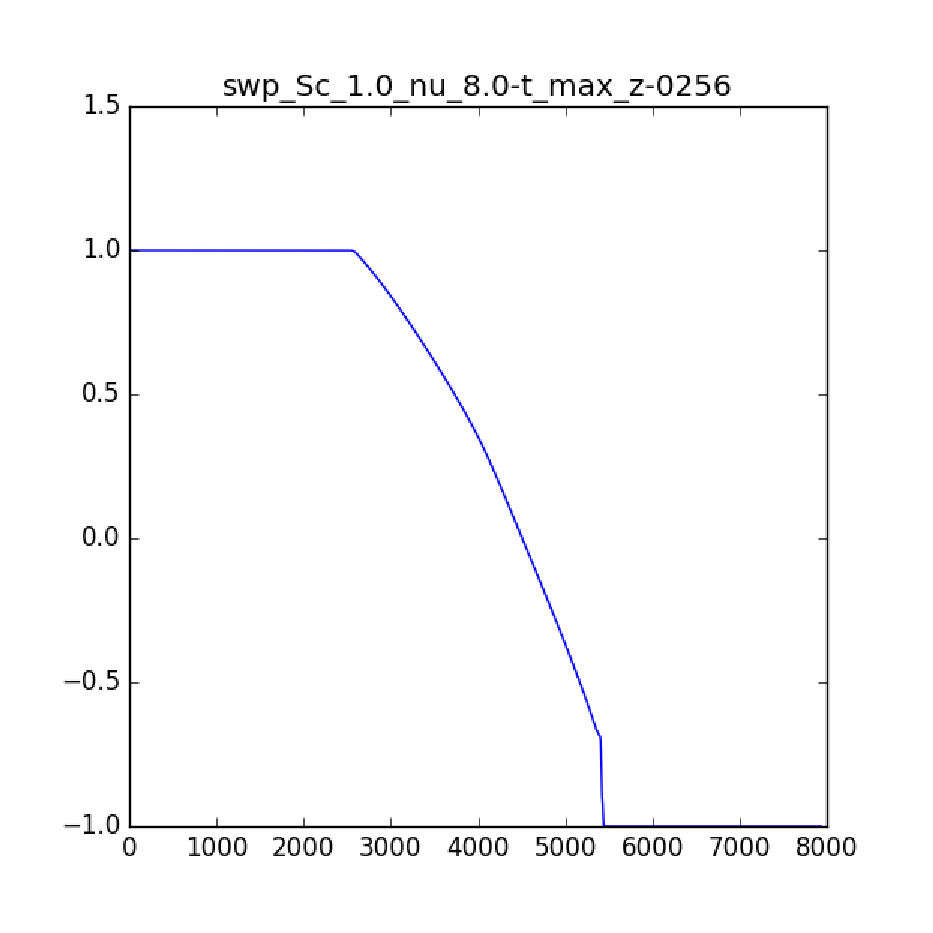
\includegraphics[width=\columnwidth]{figs/swp_Sc_1.0_nu_8.0-t_max_z-0256.eps}
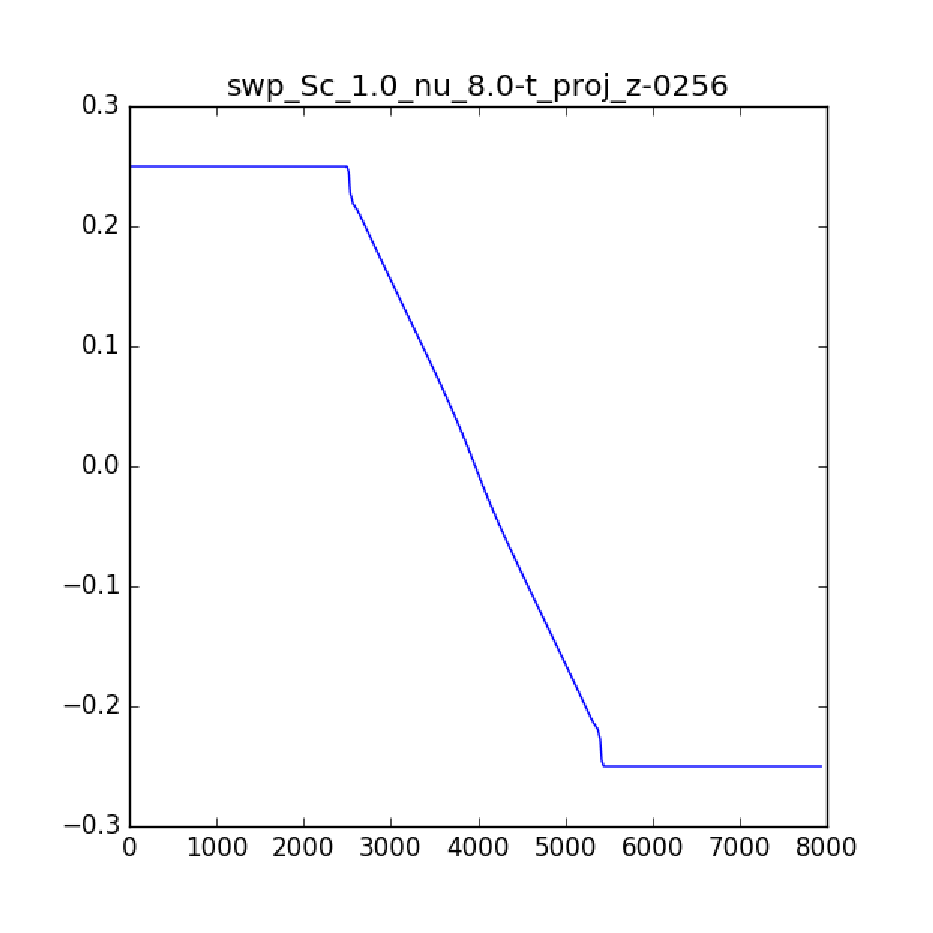
\includegraphics[width=\columnwidth]{figs/swp_Sc_1.0_nu_8.0-t_proj_z-0256.eps}
\caption{
  Spanwise max and mean of scalar field.
}
\end{figure}

\begin{figure}
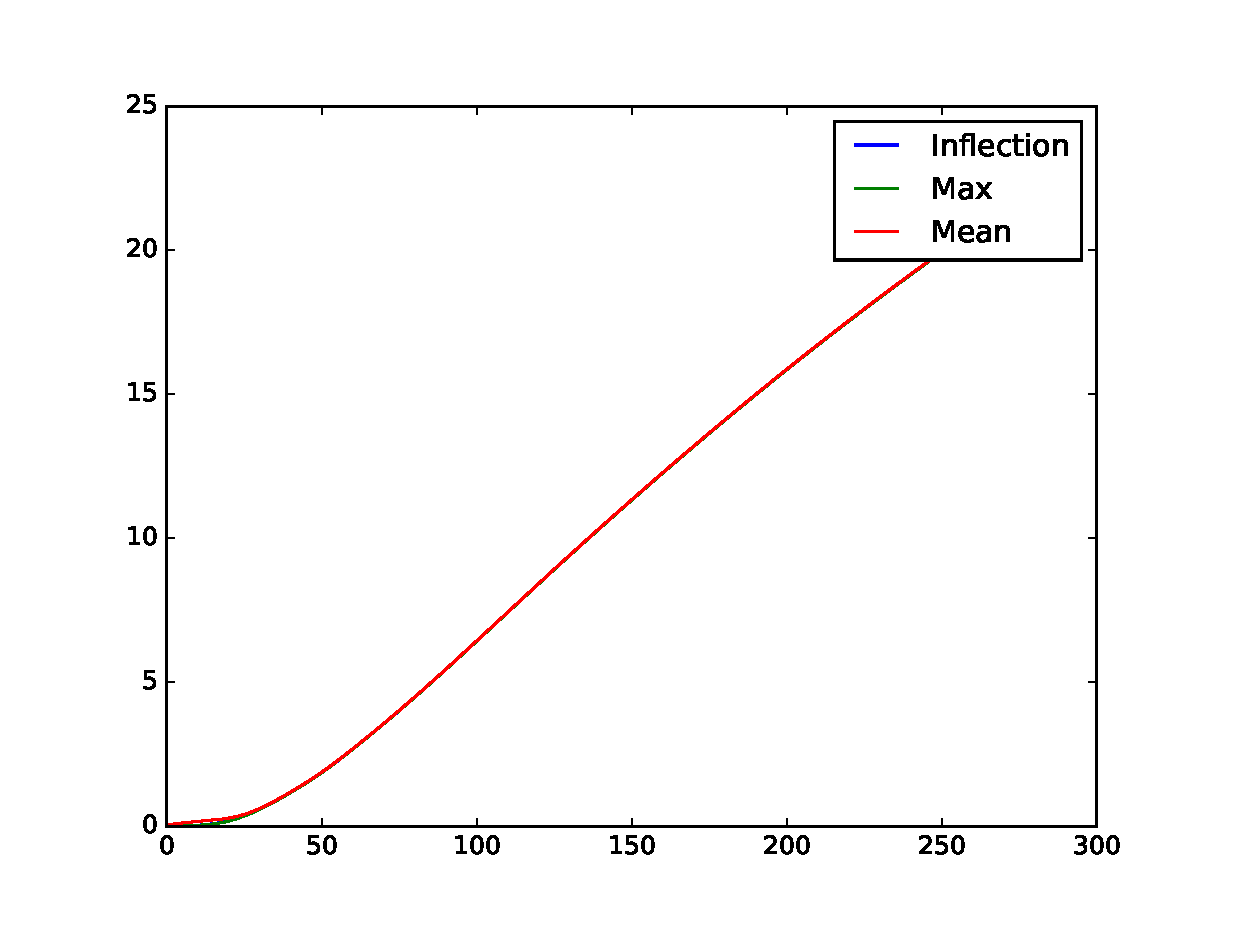
\includegraphics[width=\columnwidth]{figs/comp-height-0.0008-0.0002.eps}
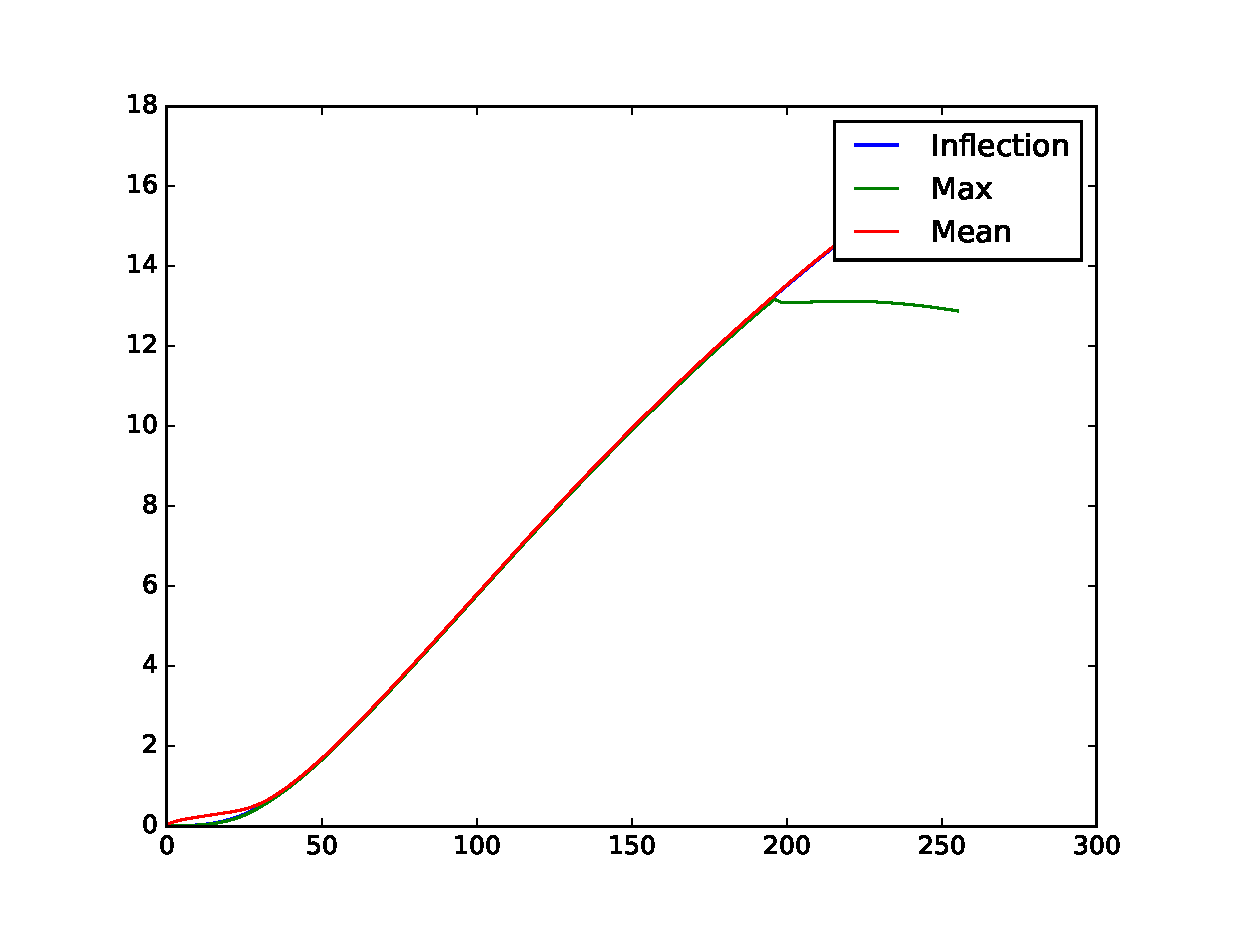
\includegraphics[width=\columnwidth]{figs/comp-height-0.0008-0.0004.eps}
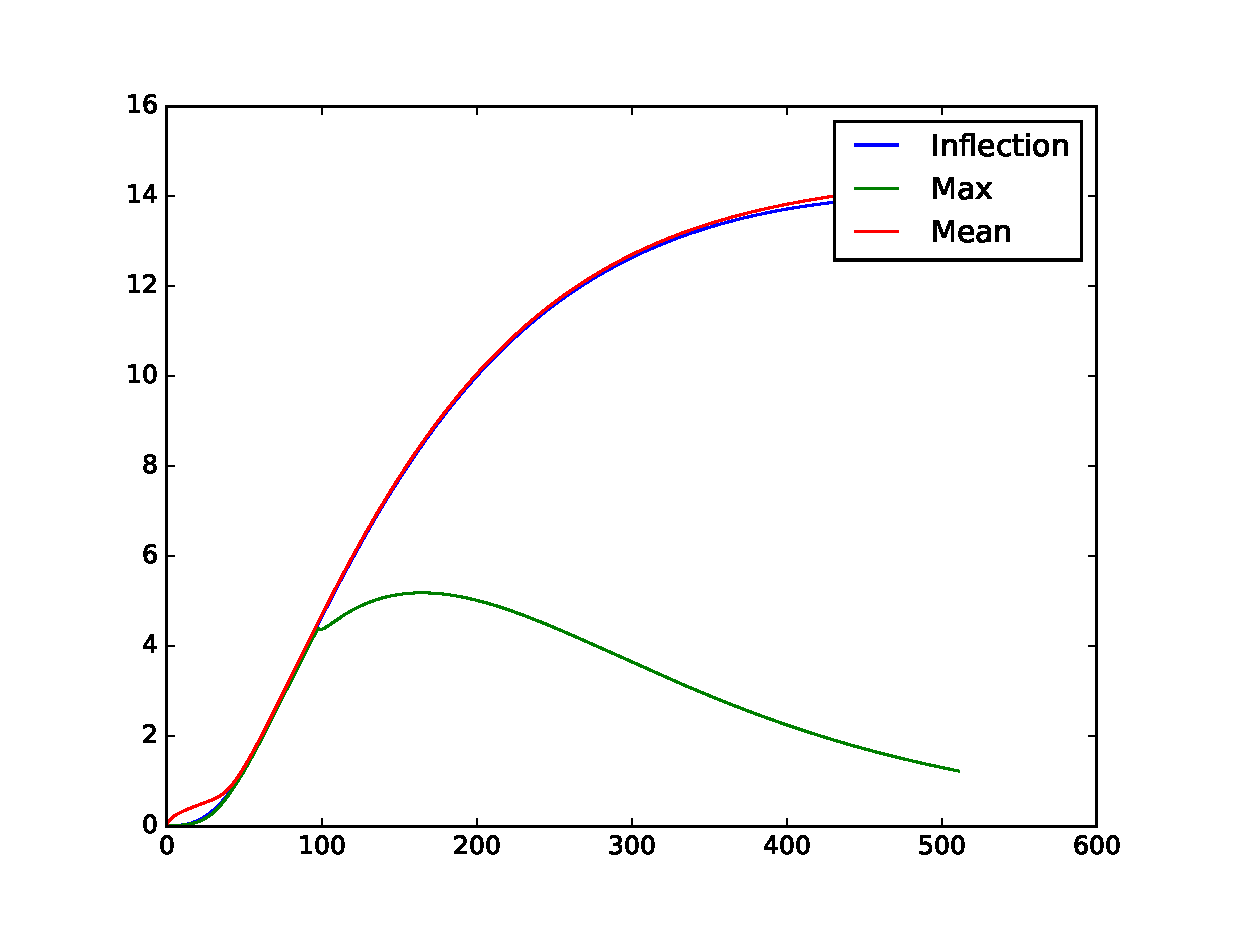
\includegraphics[width=\columnwidth]{figs/comp-height-0.0008-0.0008.eps}
\caption{
  Comparison of height metrics at $\text{Gr} = ???$ and $\text{Sc} = \{2, 4, 8\}$.
}
\end{figure}

We extract the span-wise minimum, maximum, and mean scalar values.
We are considering the miscible RTI, so the shape of the profiles is due to a combination of advection in the bubble and diffusion across the interface.
We can assume an error function-like profile across the interface at the bubble tip, but diffusion across the bubble sidewalls results in a linear profile.
To separate the definition of the bubble tip from the decreasing effective Atwood number, we introduce a new definition: the bubble tip is defined as the inflection point in the span-wise maximum scalar profile.

\subsection{Late-time behavior}



\subsection{Fitting}

The model is integrated using the variable-coefficient ordinary differential equation solver for stiff systems.
The model error is computed as the root mean square error between the integrated model and the numerical values for the bubble height.
The coefficients are fit by minimizing the model error.

The non-linear global minimization problem is solved with the covariance matrix adaptation evolution strategy (CMA-ES).
CMA-ES iteratively refines a sample distribution that evolves towards the global optimum.
Computing the model error is very inexpensive compared to the simulations, so we choose a broad initial distribution with a large population size.

